\documentclass[aspectratio=169]{beamer}
\usetheme{Madrid}
\usecolortheme{beaver}
\usepackage[utf8]{inputenc}
\usepackage[T1]{fontenc}
\usepackage{tikz}
\usepackage{amssymb}
\usepackage{graphicx}
\setbeamertemplate{navigation symbols}{}
\setbeamercolor{title}{fg=white,bg=cyan!60!black}
\setbeamercolor{frametitle}{fg=white,bg=cyan!50!black}
\setbeamercolor{block title}{bg=cyan!15,fg=black}
\setbeamercolor{block body}{bg=cyan!5,fg=black}

\title{G7 — Game States}
\subtitle{Lesson 1: The State Variable}
\author{ByteForge --- Grade 7 --- Game Maker}
\date{}

\begin{document}

\begin{frame}
    \titlepage
\end{frame}

\begin{frame}{A state is just a variable holding text}
    \Large
    What makes it a "state machine" is using IF/ELSE to draw a completely different screen depending on what the variable currently holds.

    \begin{center}
    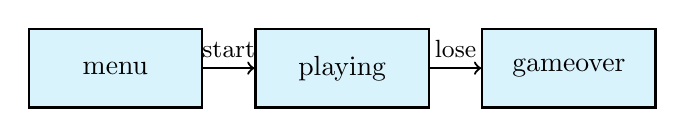
\begin{tikzpicture}[scale=0.9]

        \node[draw, thick, minimum width=2.2cm, minimum height=1cm, fill=cyan!15] (m) at (0,0) {menu};
        \node[draw, thick, minimum width=2.2cm, minimum height=1cm, fill=cyan!15] (p) at (3.2,0) {playing};
        \node[draw, thick, minimum width=2.2cm, minimum height=1cm, fill=cyan!15] (g) at (6.4,0) {gameover};
        \draw[->, thick] (m) -- (p) node[midway, above]{\small start};
        \draw[->, thick] (p) -- (g) node[midway, above]{\small lose};
    \end{tikzpicture}
    \end{center}
\end{frame}

\begin{frame}{Your Turn}
    \Large
    Open the student map, find \textbf{G7 — Game States}, and complete
    the \textbf{The State Variable} challenge --- everything you just saw, they now do themselves.
\end{frame}

\end{document}
